\documentclass[a4paper,11pt]{article}
\usepackage[spanish]{babel} % Para escribir en Espanol normal
\usepackage[utf8]{inputenc}
%\usepackage[latin1]{inputenc}
\usepackage{color}
\usepackage{array}
\usepackage{amsmath,amssymb}
\usepackage{float}
\usepackage{graphicx}
\usepackage{subfig}
\usepackage{enumerate}
\begin{document}

%Portada del Documento
\setlength{\unitlength}{1 cm} %Especificar unidad de trabajo
\thispagestyle{empty}
\begin{picture}(18,3)
\put(4,0){
\includegraphics[width=4cm,height=5cm]{logo.jpg}}
\end{picture}
\begin{center}
\textbf{{\Huge Control de Gastos }\\[0.5cm]
{\LARGE Proyecto del Primer Parcial }}\\[1.25cm]
{\Large Lenguajes de Programación}\\[2.3cm]
{\LARGE \textbf{Manual de Usuario}}\\[3.5cm]
\end{center}
{\Large Integrantes:}
\begin{itemize}
\item Vanessa Robles
\item Ricardo Campuzano
\item Ana Mora Ocaña
\end{itemize}
\begin{center}
 Ingeniería en Computación\\[0.3cm]
  ESPOL\\[1cm]
Guayaquil - \today
\end{center}
% fin de la portada

%%Tabla de Contenid
\newpage
\tableofcontents
\newpage
\section{ Introducción}

La aplicación realizada con la finalidad de ayudar al usuario a llevar un mejor control de sus facturas. Está aplicación esta dirigida  para personas naturales no obligadas a llevar contabilidad que deben cumplir que tienen problemas al momento de llevar el control de sus facturas para declaraciones de Gastos Personales en el SRI (Servicio de Rentas Internas).
La aplicación recordará al usuario las fechas que le toca hacer sus declaraciones al SRI según el informe que se ha generado al llevar la contabilidad de las facturas que se ha ido guardando.
    \subsection{ Requisitos}
\begin{itemize}
\item Eclipse IDE for Java Developers
\item Descargar el SDK de Android.
\item Plugin Android para Eclipse.
\end{itemize}


\begin{figure}[ht!]
 
   \centering
   %%----primera subfigura----
   \subfloat[]{
        \label{fig:pantalla:1}         %% Etiqueta para la primera subfigura
        
\includegraphics[width=0.42\textwidth]{img1.png}}
   \hspace{0.1\linewidth}
   %%----segunda subfigura----
   \subfloat[]{
        \label{fig:pantalla:2}         %% Etiqueta para la segunda subfigura
        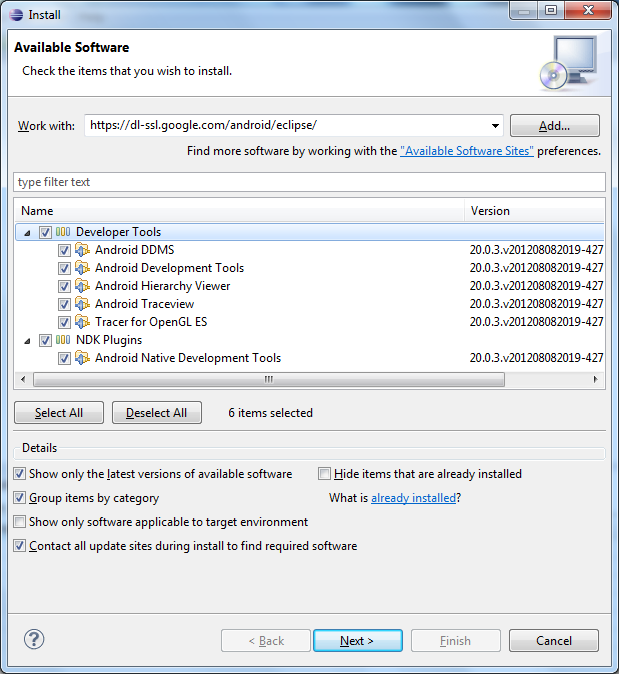
\includegraphics[width=0.42\textwidth]{img2.png}}\\[20pt]
   %%----tercera subfigura----
   \subfloat[]{
        \label{fig:pantalla:3}         %% Etiqueta para la tercera subfigura
        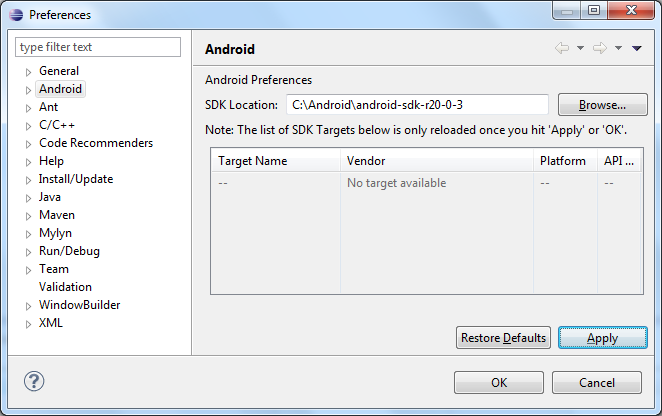
\includegraphics[width=0.42\textwidth]{img3.png}}
    
\end{figure}


\section{ Como ejecutar el proyecto}
Primero copiamos el archivo del proyecto en cualquier directorio, luego abrimos Ecplipse , seguimos los siguientes pasos:
\begin{enumerate}
\item Dar click Archivo -> Abrir Proyecto y buscamos la carpeta del proyecto en el directorio que lo guardamos.
\item Luego en la barra de herramientas dar click en ejecutar.
\end{enumerate}
     
\begin{figure}[ht!]
 
   \centering
   %%----primera subfigura----
   \subfloat[]{
        \label{fig:pantalla:1}         %% Etiqueta para la primera subfigura
        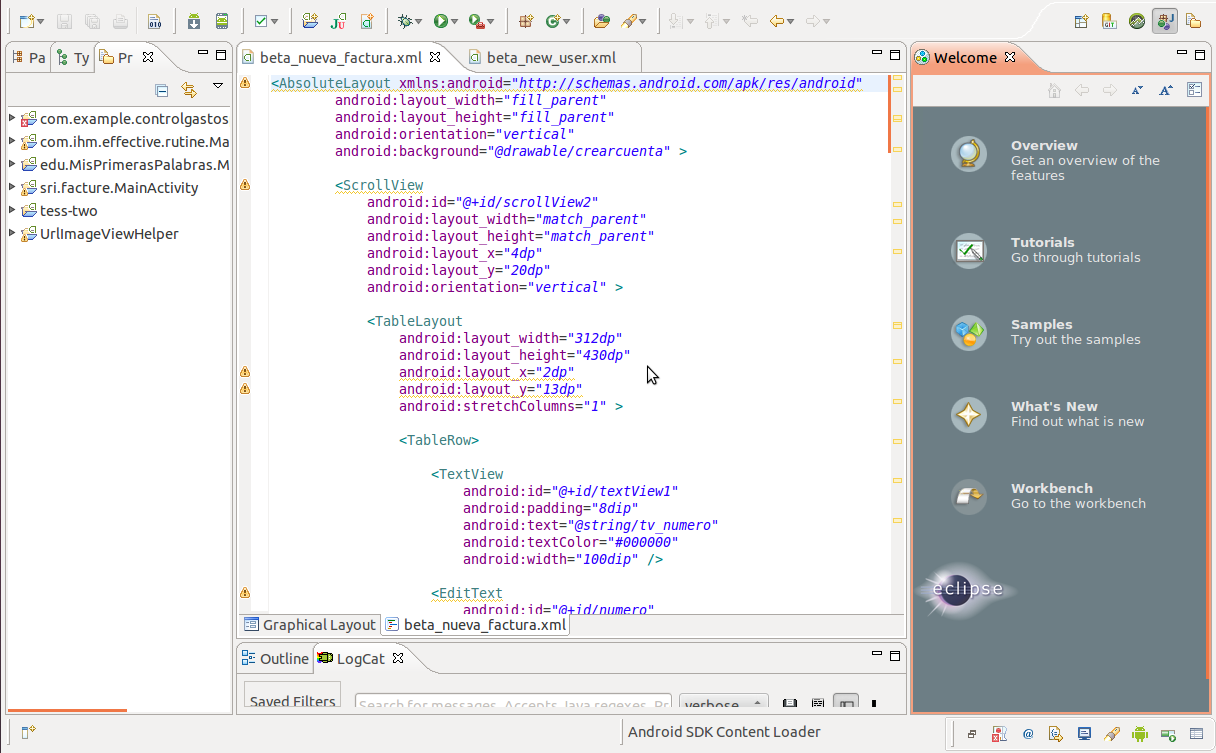
\includegraphics[width=0.42\textwidth]{img4.png}}
   \hspace{0.1\linewidth}
   %%----segunda subfigura----
   \subfloat[]{
        \label{fig:pantalla:2}         %% Etiqueta para la segunda subfigura
        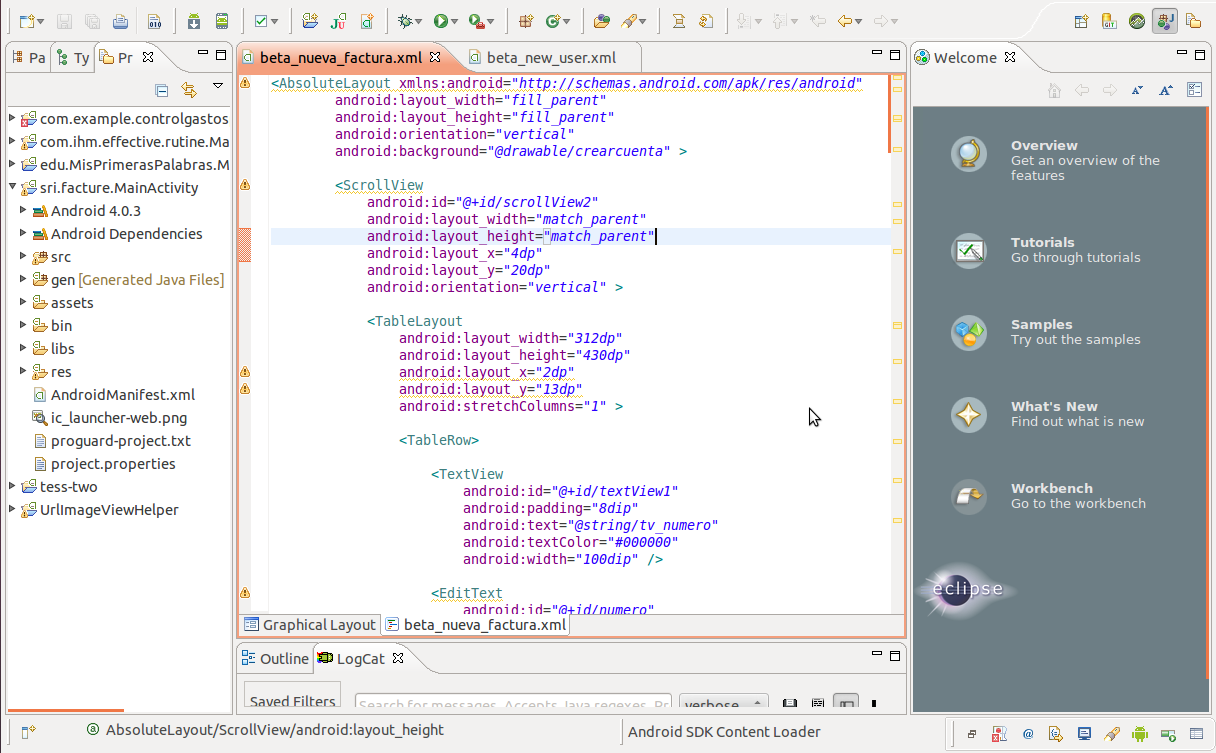
\includegraphics[width=0.42\textwidth]{img5.png}}
  
\end{figure}

 
\section{ Aplicación}
A continuación se muestran algunas imagenes de  cada una de las pantallas de la aplicación
\begin{enumerate}[a)]
     \item  El emulador cargandose
     \item Aparece el logo de la aplicacion .
     \item La primera ventana donde se ingresa el usuario y la contraseña
    \item Datos de usuario
    

\end{enumerate}

\begin{figure}[ht!]

   \centering     %%----primera subfigura----
   \subfloat[]{
        \label{fig:pantalla:1}         %% Etiqueta para la primera subfigura
        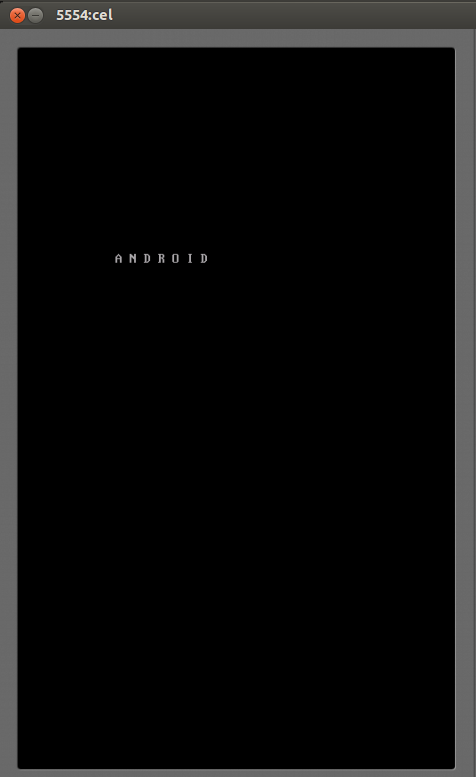
\includegraphics[width=0.42\textwidth]{img6.png}}
   \hspace{0.1\linewidth}
   %%----segunda subfigura----
   \subfloat[]{
        \label{fig:pantalla:2}         %% Etiqueta para la segunda subfigura
        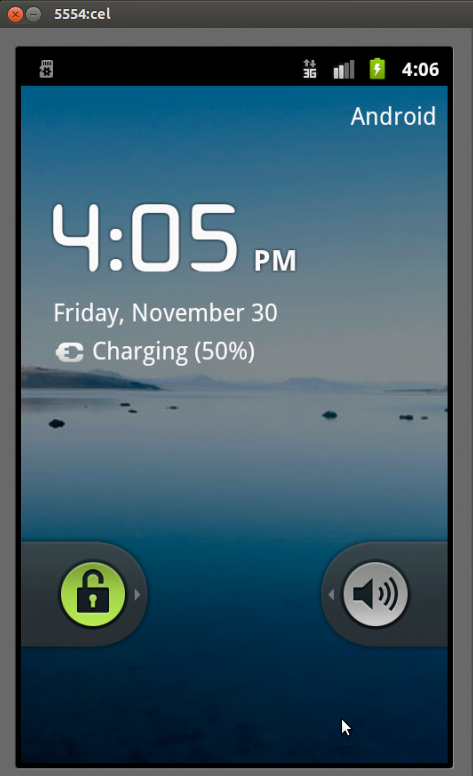
\includegraphics[width=0.42\textwidth]{img7.png}}\\[20pt]
   %%----tercera subfigura----
   \subfloat[]{
        \label{fig:pantalla:3}         %% Etiqueta para la tercera subfigura
        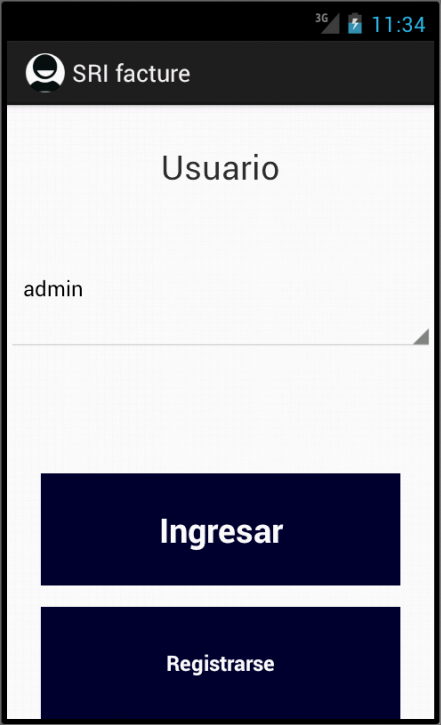
\includegraphics[width=0.42\textwidth]{img8.png}}
    \hspace{0.1\linewidth}
   %%----cuarta subfigura----
    \subfloat[]{
        \label{fig:pantalla:4}         %% Etiqueta para la cuarta subfigura
        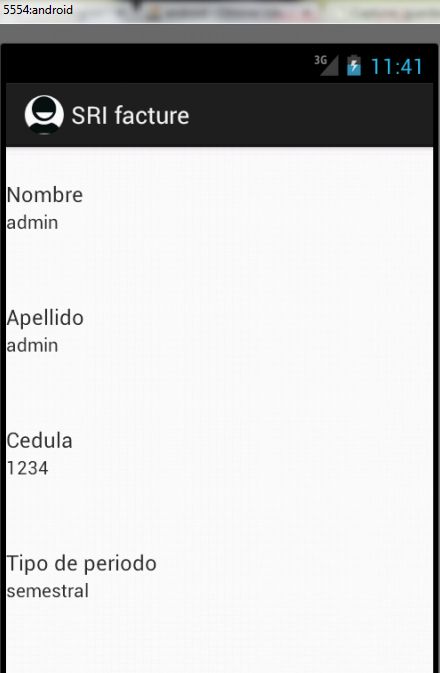
\includegraphics[width=0.42\textwidth]{img13.png}}
\end{figure}

\begin{enumerate}[a)]
       \item El menu de la aplicación.
    \item Se puede ver la pantalla donde se ingresa a abministrar factura.
       \item  En esta pantalla se muestran los diferentes valores guardados 
     \item Reporte .   
\end{enumerate}

\begin{figure}[ht!]
   \centering
   %%----primera subfigura---- \
\subfloat[]{
        \label{fig:pantalla:3}         %% Etiqueta para la tercera subfigura
        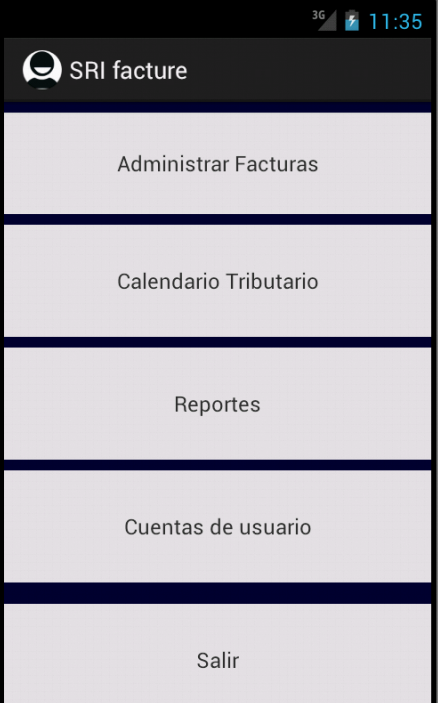
\includegraphics[width=0.42\textwidth]{img9.png}}
\hspace{0.1\linewidth}
   \subfloat[]{
        \label{fig:pantalla:1}         %% Etiqueta para la primera subfigura
        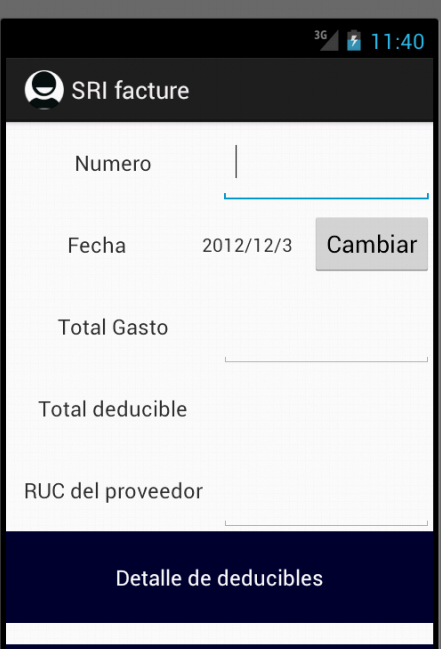
\includegraphics[width=0.42\textwidth]{img11.png}}\\[20pt]
  
   %%----segunda subfigura----
   \subfloat[]{
        \label{fig:pantalla:2}         %% Etiqueta para la segunda subfigura
        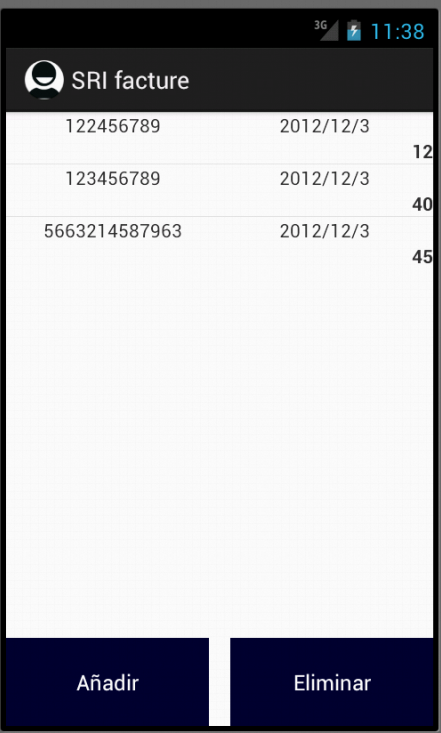
\includegraphics[width=0.42\textwidth]{img10.png}}
\hspace{0.1\linewidth}
   %%----tercera subfigura----
   \subfloat[]{
        \label{fig:pantalla:3}         %% Etiqueta para la tercera subfigura
        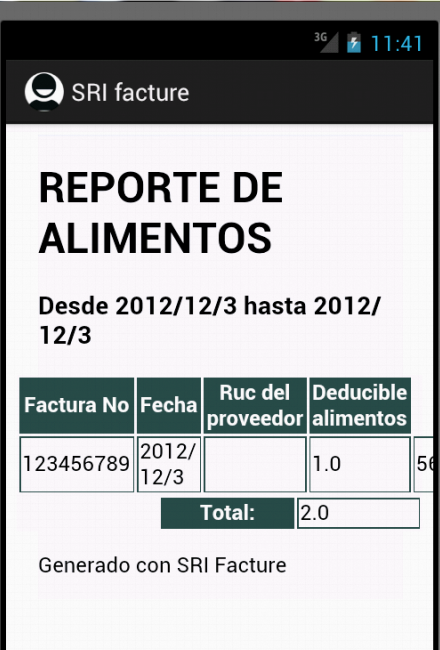
\includegraphics[width=0.42\textwidth]{img12.png}}
   
\end{figure}

\end {document}

